\documentclass[../main.tex]{subfiles}
\begin{document}

\section{Model performance on dataset without exclusion of features after AKI development}


\subsection{Model performance on dataset without new features}

 \begin{figure}[H]
    \centering
    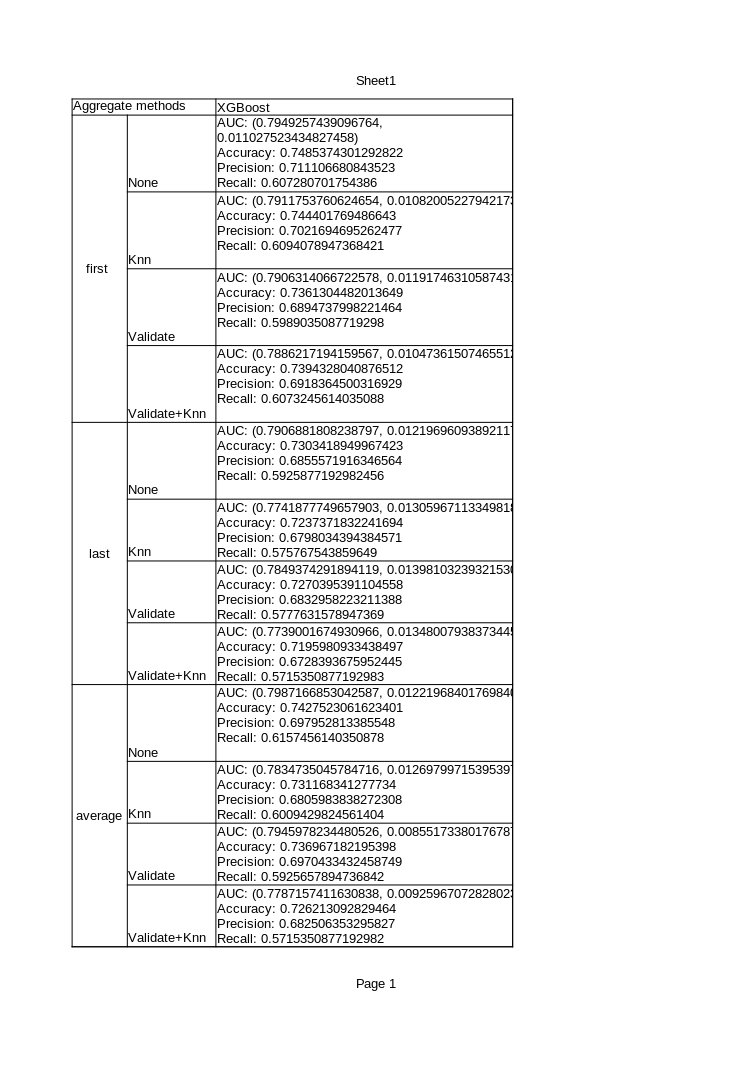
\includegraphics[width=\textwidth]{Figure/KidneyResultNoLimit_XGBoost.png}
    \caption{Performance of XGBoost}
    \label{fig:KidneyResultNoLimit_XGBoost}
\end{figure}

 \begin{figure}[H]
    \centering
    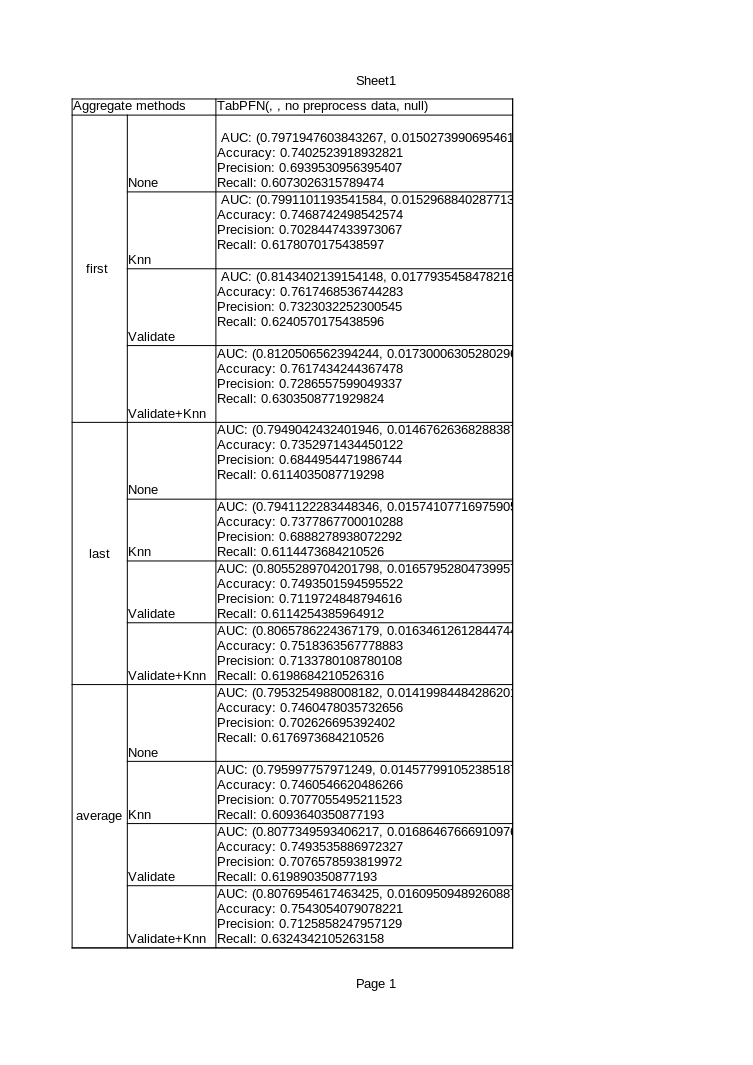
\includegraphics[width=\textwidth]{Figure/KidneyResultNoLimit_TabPFN.png}
    \caption{Performance of TabPFN}
    \label{fig:KidneyResultNoLimit_TabPFN}
\end{figure}

 \begin{figure}[H]
    \centering
    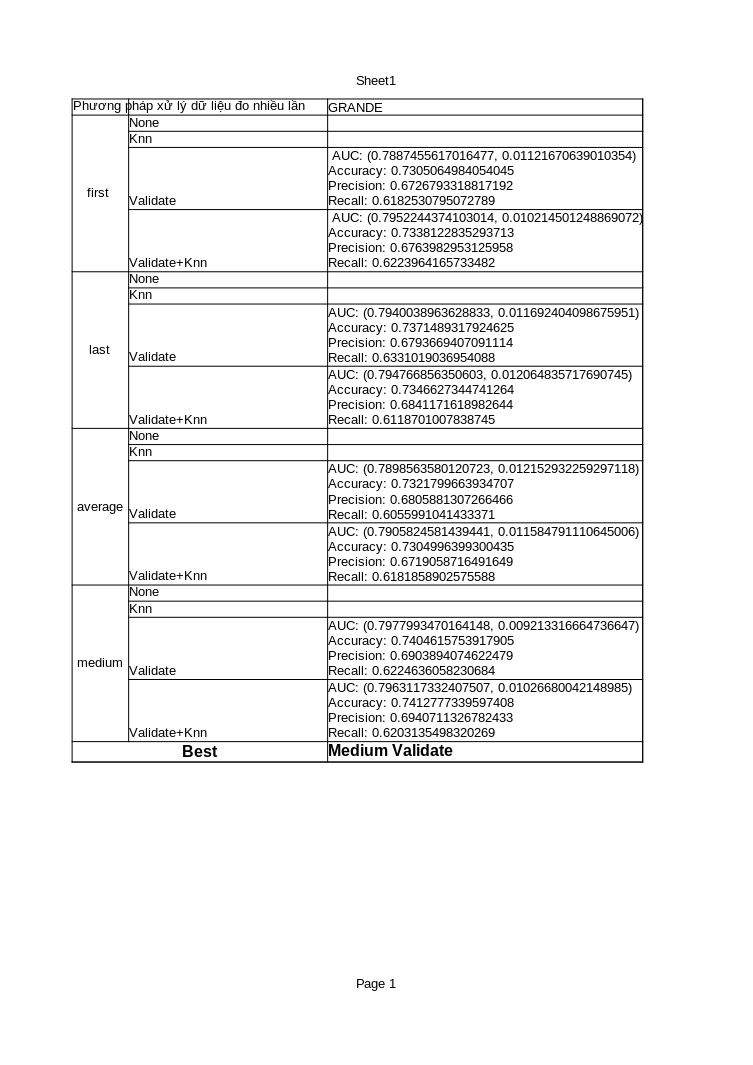
\includegraphics[width=\textwidth]{Figure/KidneyResultNoLimit-new_GRANDE.png}
    \caption{Performance of GRANDE}
    \label{fig:KidneyResultNoLimit-new_GRANDE}
\end{figure}


\subsection{Model performance on dataset without new features}

 \begin{figure}[H]
    \centering
    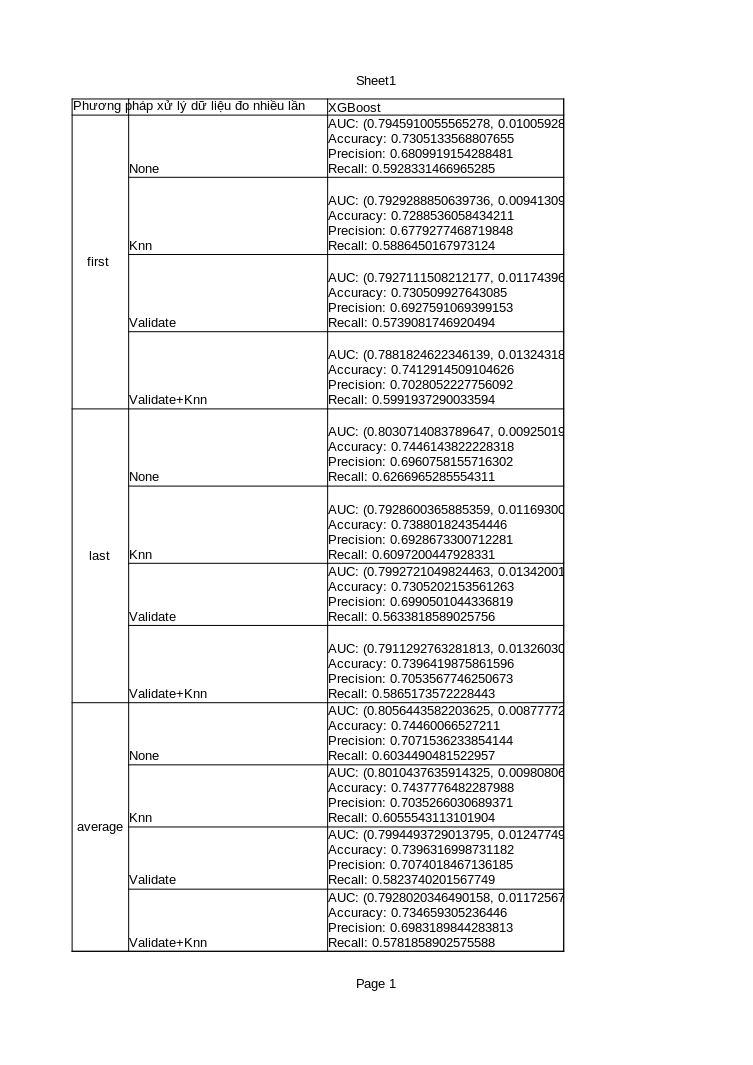
\includegraphics[width=\textwidth]{Figure/KidneyResultNoLimit-new_XGBoost.png}
    \caption{Performance of XGBoost}
    \label{fig:KidneyResultNoLimit-new_XGBoost}
\end{figure}

 \begin{figure}[H]
    \centering
    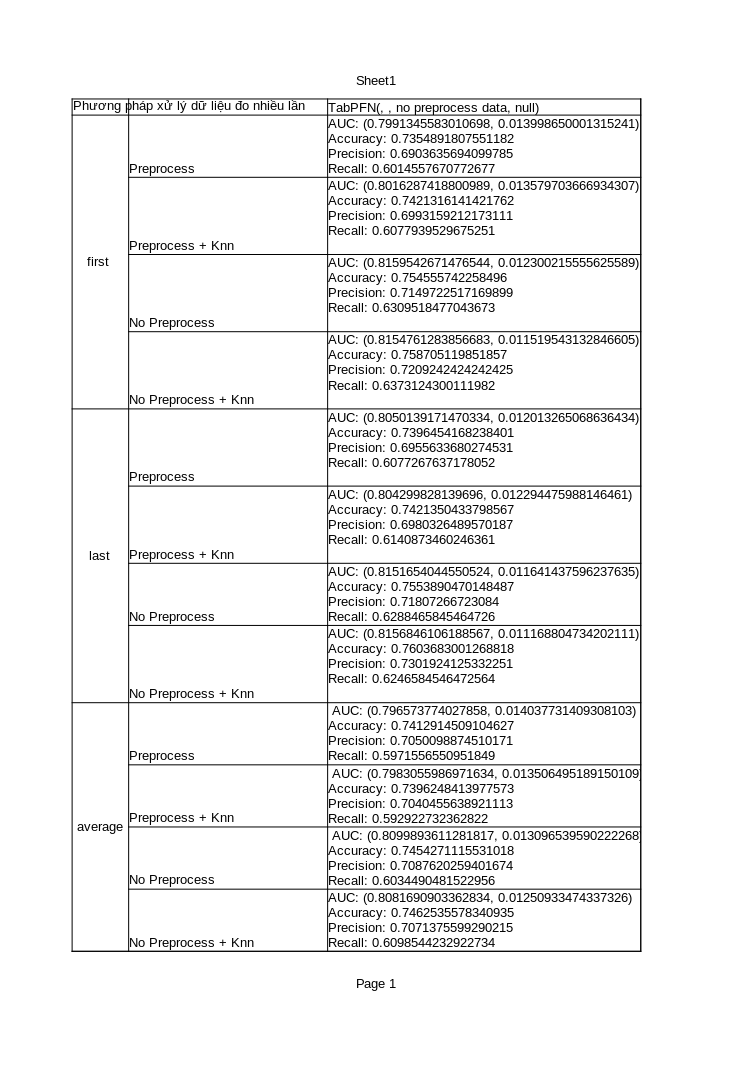
\includegraphics[width=\textwidth]{Figure/KidneyResultNoLimit-new_TabPFN.png}
    \caption{Performance of TabPFN}
    \label{fig:KidneyResultNoLimit-new_TabPFN}
\end{figure}

 \begin{figure}[H]
    \centering
    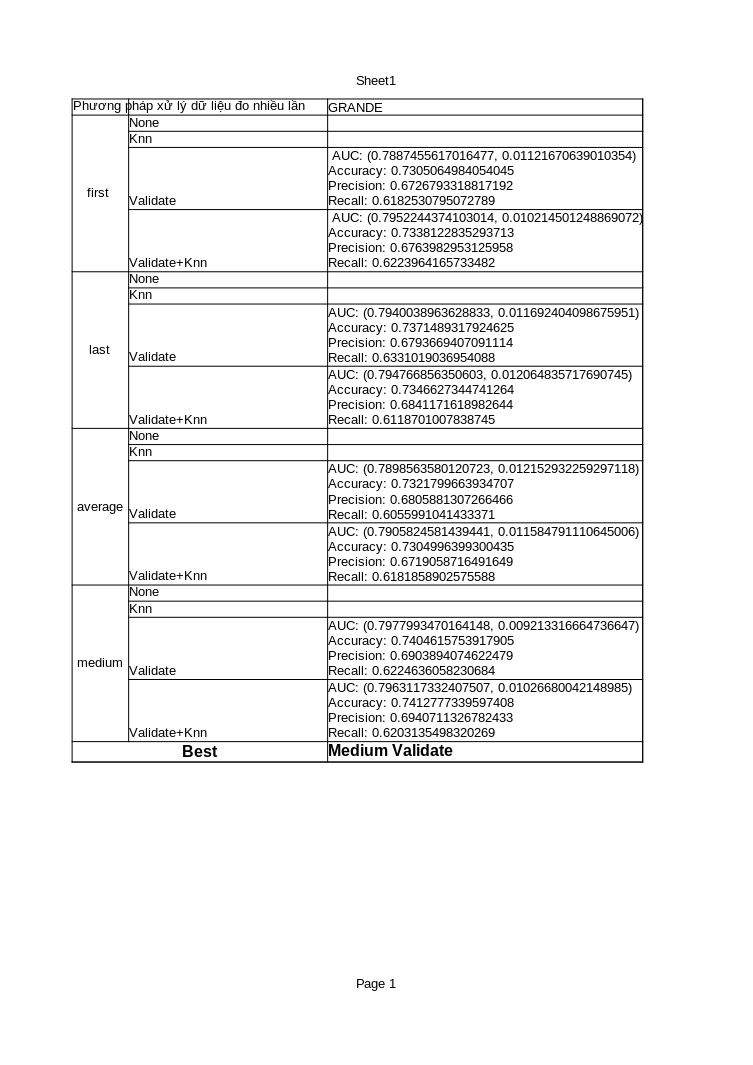
\includegraphics[width=\textwidth]{Figure/KidneyResultNoLimit-new_GRANDE.png}
    \caption{Performance of GRANDE}
    \label{fig:KidneyResultNoLimit-new_GRANDE}
\end{figure}


\section{Model performance on dataset excluding features after AKI development}


\subsection{Model performance on dataset without new features}

 \begin{figure}[H]
    \centering
    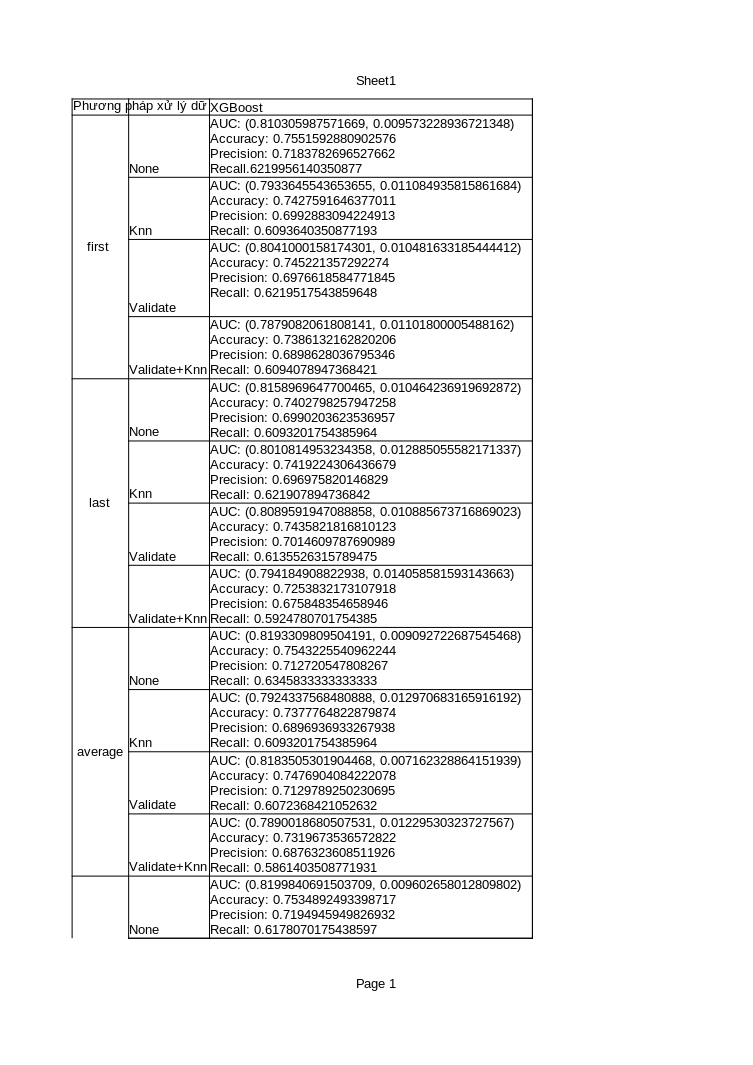
\includegraphics[width=\textwidth]{Figure/KidneyResultLimit_XGBoost.png}
    \caption{Performance of XGBoost}
    \label{fig:KidneyResultLimit_XGBoost}
\end{figure}

 \begin{figure}[H]
    \centering
    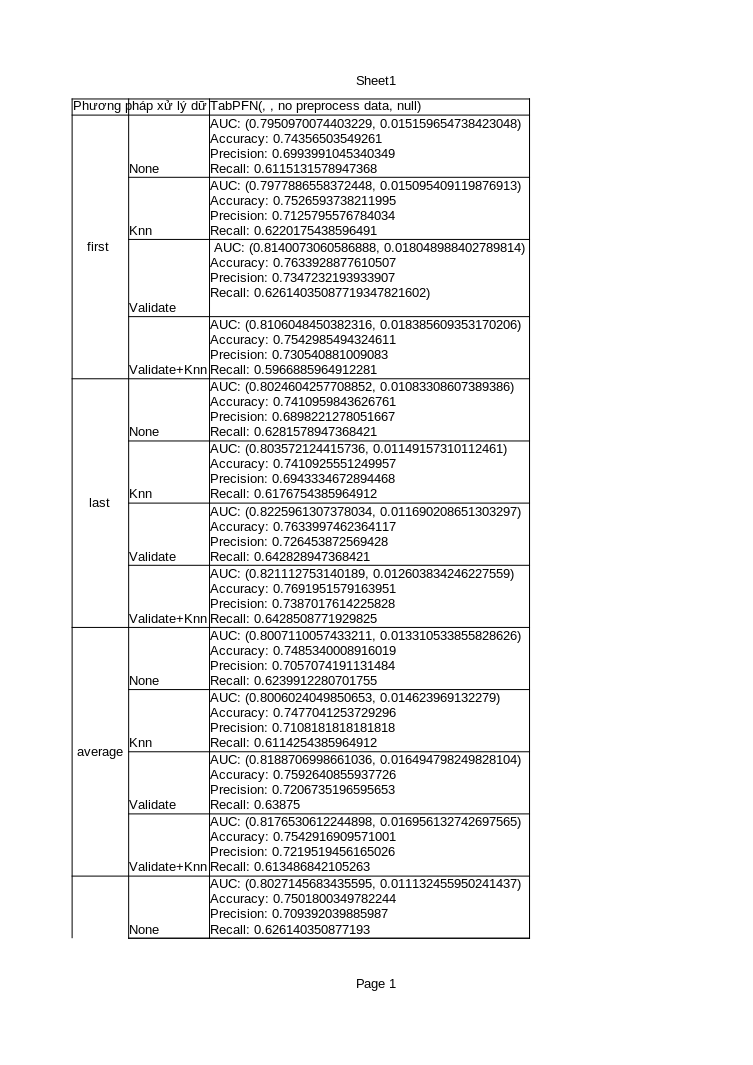
\includegraphics[width=\textwidth]{Figure/KidneyResultLimit_TabPFN.png}
    \caption{Performance of TabPFN}
    \label{fig:KidneyResultLimit_TabPFN}
\end{figure}

 \begin{figure}[H]
    \centering
    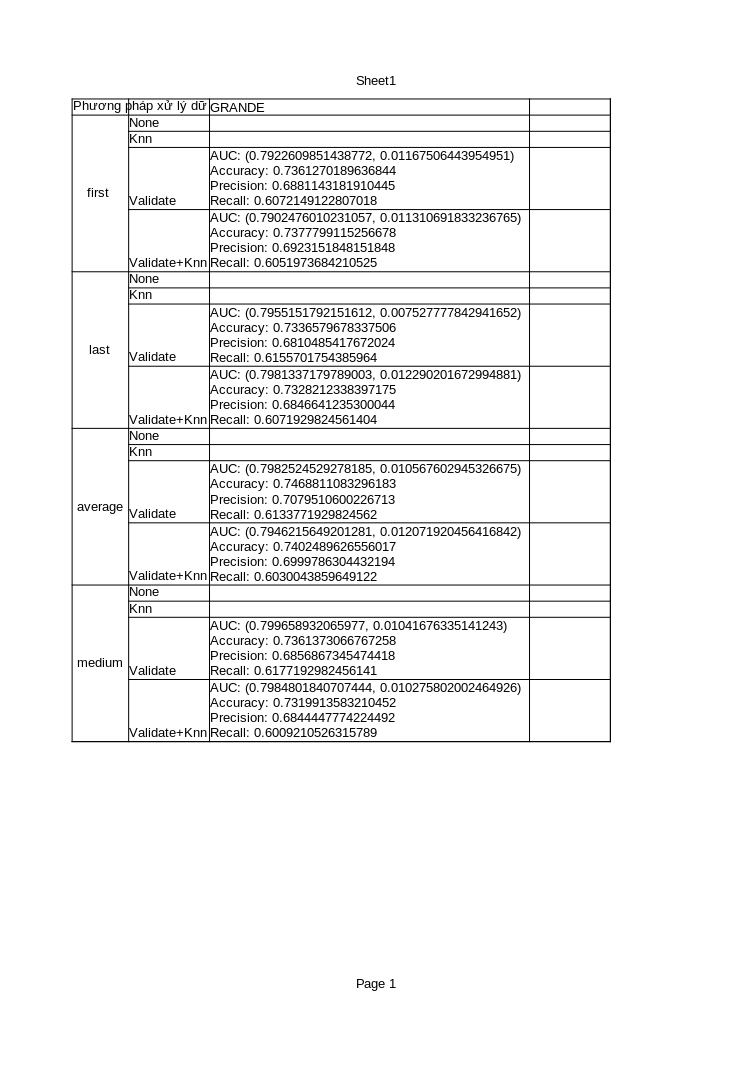
\includegraphics[width=\textwidth]{Figure/KidneyResultLimit_GRANDE.png}
    \caption{Performance of GRANDE}
    \label{fig:KidneyResultLimit_GRANDE}
\end{figure}


\subsection{Model performance on dataset without new features}

 \begin{figure}[H]
    \centering
    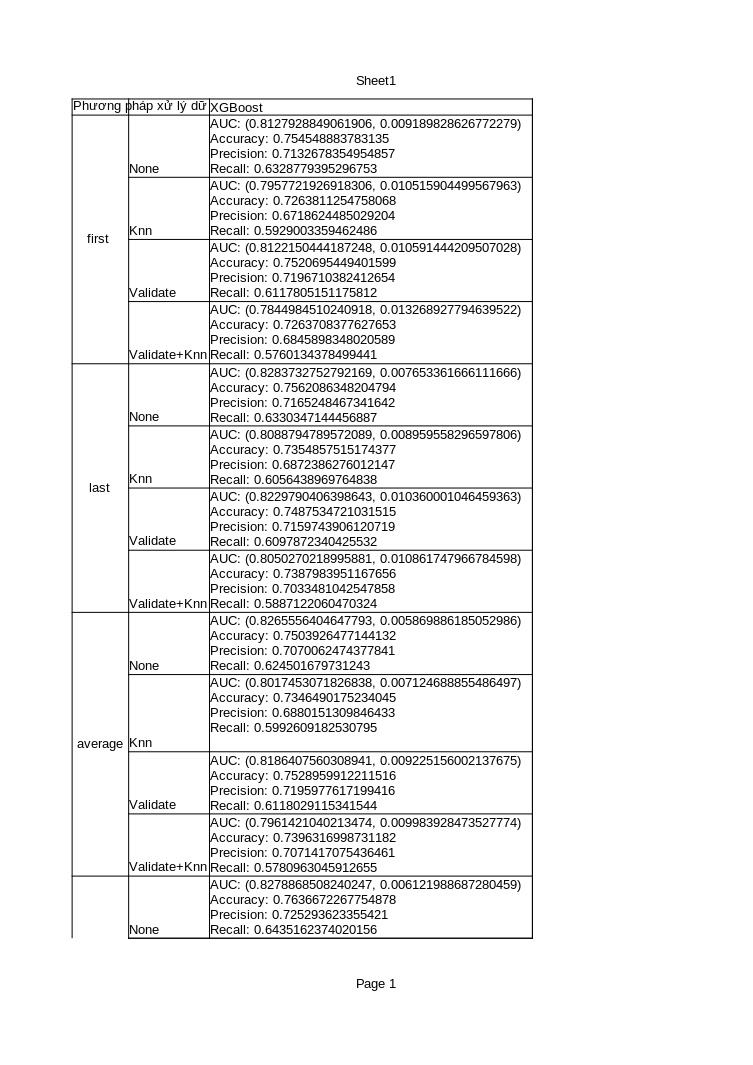
\includegraphics[width=\textwidth]{Figure/KidneyResultLimit-new_XGBoost.png}
    \caption{Performance of XGBoost}
    \label{fig:KidneyResultLimit-new_XGBoost}
\end{figure}

 \begin{figure}[H]
    \centering
    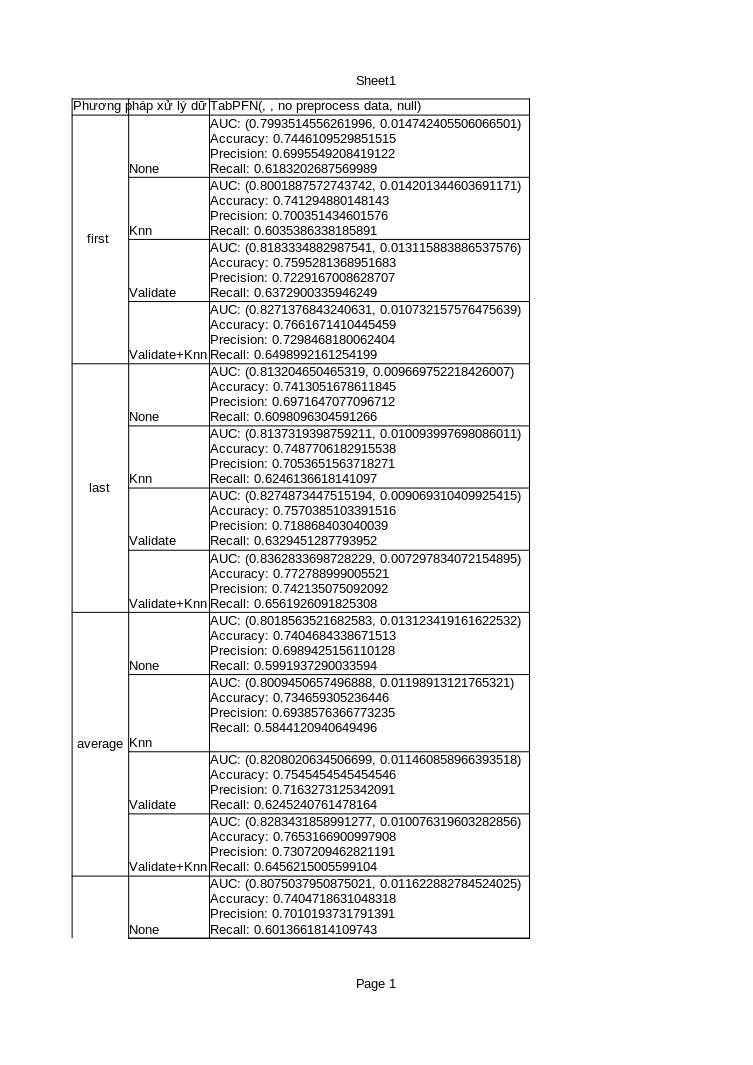
\includegraphics[width=\textwidth]{Figure/KidneyResultLimit-new_TabPFN.png}
    \caption{Performance of TabPFN}
    \label{fig:KidneyResultLimit-new_TabPFN}
\end{figure}

 \begin{figure}[H]
    \centering
    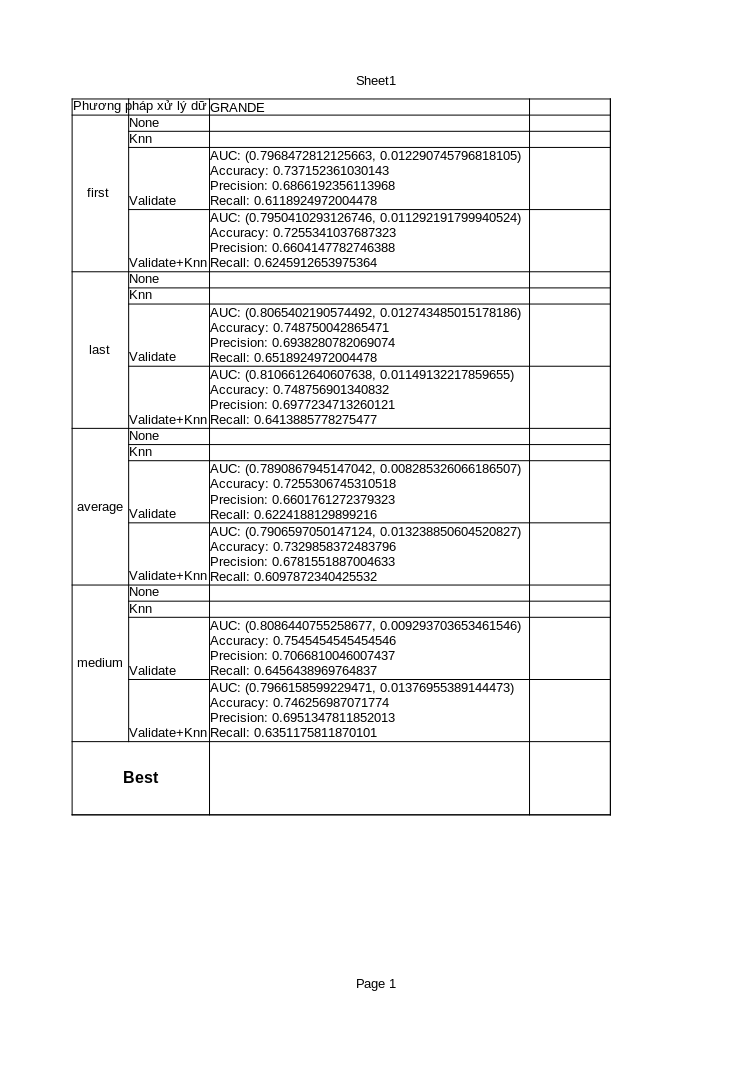
\includegraphics[width=\textwidth]{Figure/KidneyResultLimit-new_GRANDE.png}
    \caption{Performance of GRANDE}
    \label{fig:KidneyResultLimit-new_GRANDE}
\end{figure}



\end{document}